\documentclass[11pt,twoside]{article}
% \input{hwheader.tex}

%\documentclass[11pt,twoside]{article}
\usepackage[nonamelimits]{amsmath}
\usepackage{amssymb, amsthm}

\setlength{\oddsidemargin}{0 in}
\setlength{\evensidemargin}{0 in}
\setlength{\topmargin}{-0.6 in}
\setlength{\textwidth}{6.5 in}
\setlength{\textheight}{8.5 in}
\setlength{\headheight}{0.5 in}
\setlength{\headsep}{0.5 in}
\setlength{\parindent}{0 in}
\setlength{\parskip}{0.1 in}


%%% SETS
\newcommand\Z{\mbox{$\mathbb Z$}}
\newcommand\N{\mbox{$\mathbb N$}}
\newcommand\R{\mbox{$\mathbb R$}}
\newcommand\F{\mbox{$\mathbb F$}}
\def\B{\{0,1\}}
\def\cond{\mid}

%%% FUNCTIONS
\providecommand\floor[1]{\lfloor#1\rfloor}
\providecommand\ceil[1]{\lceil#1\rceil}
\providecommand\blog[1]{\log_2\ceil{#1}}
\providecommand\abs[1]{\lvert#1\rvert}
\providecommand\bigabs[1]{\bigl\lvert#1\bigr\rvert}

\def\co{{\rm co}}
\def\avg{{\rm Avg}}
\def\heur{{\rm Heur}}

%%% THEOREM TYPE ENVIRONMENTS
\newtheorem{theorem}{Theorem}
\newtheorem{lemma}[theorem]{Lemma}
\newtheorem{corollary}[theorem]{Corollary}
\newtheorem{proposition}[theorem]{Proposition}
\newtheorem{claim}[theorem]{Claim}
\newtheorem{exercise}{Exercise}
\newtheorem{conjecture}{Conjecture}
\newtheorem{example}{Example}
\newtheorem{remark}{Remark}
\newtheorem{definition}[theorem]{Definition}



%%% HEADINGS
\newcommand{\homework}[1]{
   \pagestyle{myheadings}
   \thispagestyle{plain}
   \newpage
   \setcounter{page}{1}
   \noindent
   \classname \hfill \mbox{\updatedday} \\
   \instname \hfill \mbox{\duedate}
   \rule{6.5in}{0.5mm}
   \vspace*{-0.1 in}
}


\newcommand{\problem}[1]{\section*{Problem #1}}


\renewcommand{\labelenumi}{(\alph{enumi})}
\renewcommand{\labelenumii}{(\roman{enumii})}

%%% DEFINITIONS
\def\classname{CSCI-SHU 220: Algorithms @ NYU Shanghai}


%%% INSTRUCTIONS
\raggedbottom 


\usepackage[pdftex]{graphicx}
\usepackage{pgf,tikz}
\usetikzlibrary{shapes,arrows,automata}

\usepackage{listings}
\usepackage{xcolor}
\lstset { %
    language=C++,
    backgroundcolor=\color{black!5}, % set backgroundcolor
    basicstyle=\footnotesize,% basic font setting
}

\newcommand\includefa[1]{\begin{center}\includegraphics[scale=0.5]{#1}\end{center}}


\def\updatedday{Last Updated: October 16, 2020}
\def\duedate{Due Date: November 9, 2020, 11:00pm}

\newenvironment{solution}{{\par\noindent\it Solution.}}{}

\def\instname{Homework 3}

\begin{document}
\homework{3}

You are allowed to discuss with others but not allow to use references other than the course notes and reference books. Please list your collaborators for each questions. Write your own solutions and make sure you understand them. 

There are 55 marks in total (including the bonus). The full mark of this homework is 50.  

Enjoy :). 

\textit{Please specify the following information before submission}:
\begin{itemize}
    \item Your Name: Liangzu Peng%  (put your name here)
    \item Your NetID: lp2528% (put your NetID here)
    \item Collaborators: % (write down the names of your collaborators if any).
\end{itemize}

\problem{1: Interval scheduling [10 marks]} 
In the problem of interval scheduling, suppose that instead of always selecting the first interval to finish, we select the last interval to start that is compatible with all previously selected intervals. Describe how this approach is a greedy algorithm, and prove that it yields an optimal solution.

\begin{solution}
\textbf{Please write down your solution to Problem 1 here.}
\end{solution}

\problem{2: The weighted total completion time [12 marks]}
Suppose that there are $n$ jobs labeled as $1,2,\dots,n$. Each job $j$ has length $\ell_j$, which is the amount of time required to process the job. Also, each job $j$ has a weight $w_j$, with higher weights corresponding to jobs of higher priority. A schedule $\sigma$ specifies an order in which to process the jobs. For example, if $n=3$ and $\sigma=(2,1,3)$, then we first process job $2$, then job 1, and finally job $3$. The completion time $C_j(\sigma)$ of a job $j$ in a schedule $\sigma$ is the sum of the lengths of the jobs preceding $j$ in $\sigma$, plus the length of $j$ itself. Our goal is to design an algorithm that takes as inputs the weights $w_1,\dots,w_n$ and the lengths $\ell_1,\dots,\ell_n$, and outputs a schedule $\sigma^*$ which minimizes the following objective function:
\begin{align}
    \min\limits_{\sigma} \sum_{j=1}^n w_jC_j(\sigma).
\end{align}
\begin{enumerate}
    \item (4 marks) Consider the greedy algorithm that schedules the jobs in decreasing order of $w_j-\ell_j$. Is this greedy algorithm optimal (in the sense that it always find a minimizer of the above objective function)? Prove or disprove it.
    
    % Prove that this algorithm is incorrect, that is, it can not always find a minimizer of the above objective function.
    \item (8 marks) Consider the greedy algorithm that schedules the jobs in decreasing order of $w_j/\ell_j$. Is this greedy algorithm optimal? Prove or disprove it.
\end{enumerate}

\begin{solution}
\textbf{Please write down your solution to Problem 2 here.}
\end{solution}


\problem{3: Merging lists [11 marks]}
Consider the problem of merging $k$ sorted lists $L_1,\dots,L_k$ of sizes $n_1,\dots,n_k$. Let $n=n_1+\cdots+n_k$.
\begin{enumerate}
    \item (3 marks) Consider the algorithm that repeatedly merge take two lists from $L_1,\dots,L_k$ and merge them so that we 
    obtain a single sorted list after $k-1$ merges. What is the complexity of this algorithm? Assume that merging two lists of sizes $\ell_1$ and $\ell_2$ respectively entails a cost $\ell_1+\ell_2$. What is the cost of this algorithm?
    \item (8 marks) The above cost would depend on the order in which the lists are taken and merged. For example, when $k=3$, there are six possible orders for merging: $(1,2,3)$, $(1,3,2)$, $(2,1,3)$, $(2,3,1)$, $(3,1,2)$, and $(3,2,1)$. Here $(1,2,3)$ means that we first merge $L_1$ and $L_2$, and the resulting list is taken to be merged with $L_3$. It is not hard to observe that the orders $(1,2,3)$ and $(2,1,3)$ have the same cost, and that all these orders give three potentially different costs, say $2n-n_1$, $2n-n_2$, and $2n-n_3$. One can verify that the minimum cost is $2n-\max\{n_1,n_2,n_3\}$, attained when we first merge the two shortest lists. Based on this discussion, give a greedy algorithm to merge the lists, and prove that it is optimal in the sense that it entails the smallest possible cost.
\end{enumerate}
\begin{solution}
\textbf{Please write down your solution to Problem 3 here.}
\end{solution}



\problem{4: Guards for the farmer [11 marks]}
A farmer who grows watermelons wants to put guards on her warehouse in the time interval $[0,M]$. There are $n$ guards and the $i$-th guard can work during time interval $[s_i,f_i]$. The farmer wants to hire a minimum number of guards, such that in any time point $t\in[0,M]$ there is at least one guard whose time interval covers $t$, i.e., $t\in[s_i,f_i]$. For example, for $M=15$ and $n=6$, the guards can work at time intervals
$[0,3],[5,9],[9,13],[0,7],[10,15],$ and $[7,12]$, there is a solution of size $3$ by hiring $3$ guards who work at times: $[0,7],[7,12],$ and $[10,15]$.
\begin{enumerate}
    \item (3 marks) under what conditions on the time intervals the farmer can not hire a minimum number of guards, such that in any time point $t\in[0,M]$ there is at least one guard whose time interval covers $t$, i.e., $t\in[s_i,f_i]$?
    \item (8 marks) Assume that it is possible for the farmer to hire such a minimum number of guards. Help the farmer design a greedy algorithm to hire, suggest an implementation of complexity $O(n\log n)$, and prove its correctness.
\end{enumerate}

\begin{solution}
\textbf{Please write down your solution to Problem 4 here.}
\end{solution}

\problem{5: Oh! Beautiful Spring! [11 marks]}

Happy Rotter loves his life, so he spends one of his weekends in the park enjoying the brilliant spring time. However, he comes along with two problems during his trip. Can you help him solve them?

\begin{enumerate}
	\item (3 marks) On the way the the park Happy Rotter heard many birds singing vividly, and it seems that the birds sang with a pattern!
    Assume different birds $a, b, c, d, e, f, g$ sing with frequencies $0.15, 0.23, 0.07, 0.18, 0.09, 0.11, 0.17$ respectively, show an optimal binary decoding tree for this pattern.
	Just draw the tree and label the leaves.
    No explanations or intermediate calculations required.

	\item (8 marks) Along the long long road in the park many cherry trees are planted, with locations $x_1 \leq x_2 \leq ... \leq x_n$.
	Now all the trees have blossomed and the view is brilliant!
	The park staffs set up stalls along the road to serve visitors, but Happy Rotter is not very satisfied -- they are either too far away from the trees or too close to each other.
	There must be a better way to arrange these stalls.

	Assume that each stall can serve visitors within $k$ miles, and you may consider that the visitors only gather nearby the cherry trees.
	Your goal is to serve more visitors using fewer stalls.
	Given $x_1 \leq ... \leq x_n$ and $k$, design an efficient algorithm to output a minimum set of stall locations to achieve the goal.
	State your algorithm clearly.
	Provide a brief explanation of its correctness.
	You will get full marks if the time complexity is $O(n)$ and the explanation is good.

	\begin{figure}[htbp]
		\centering
		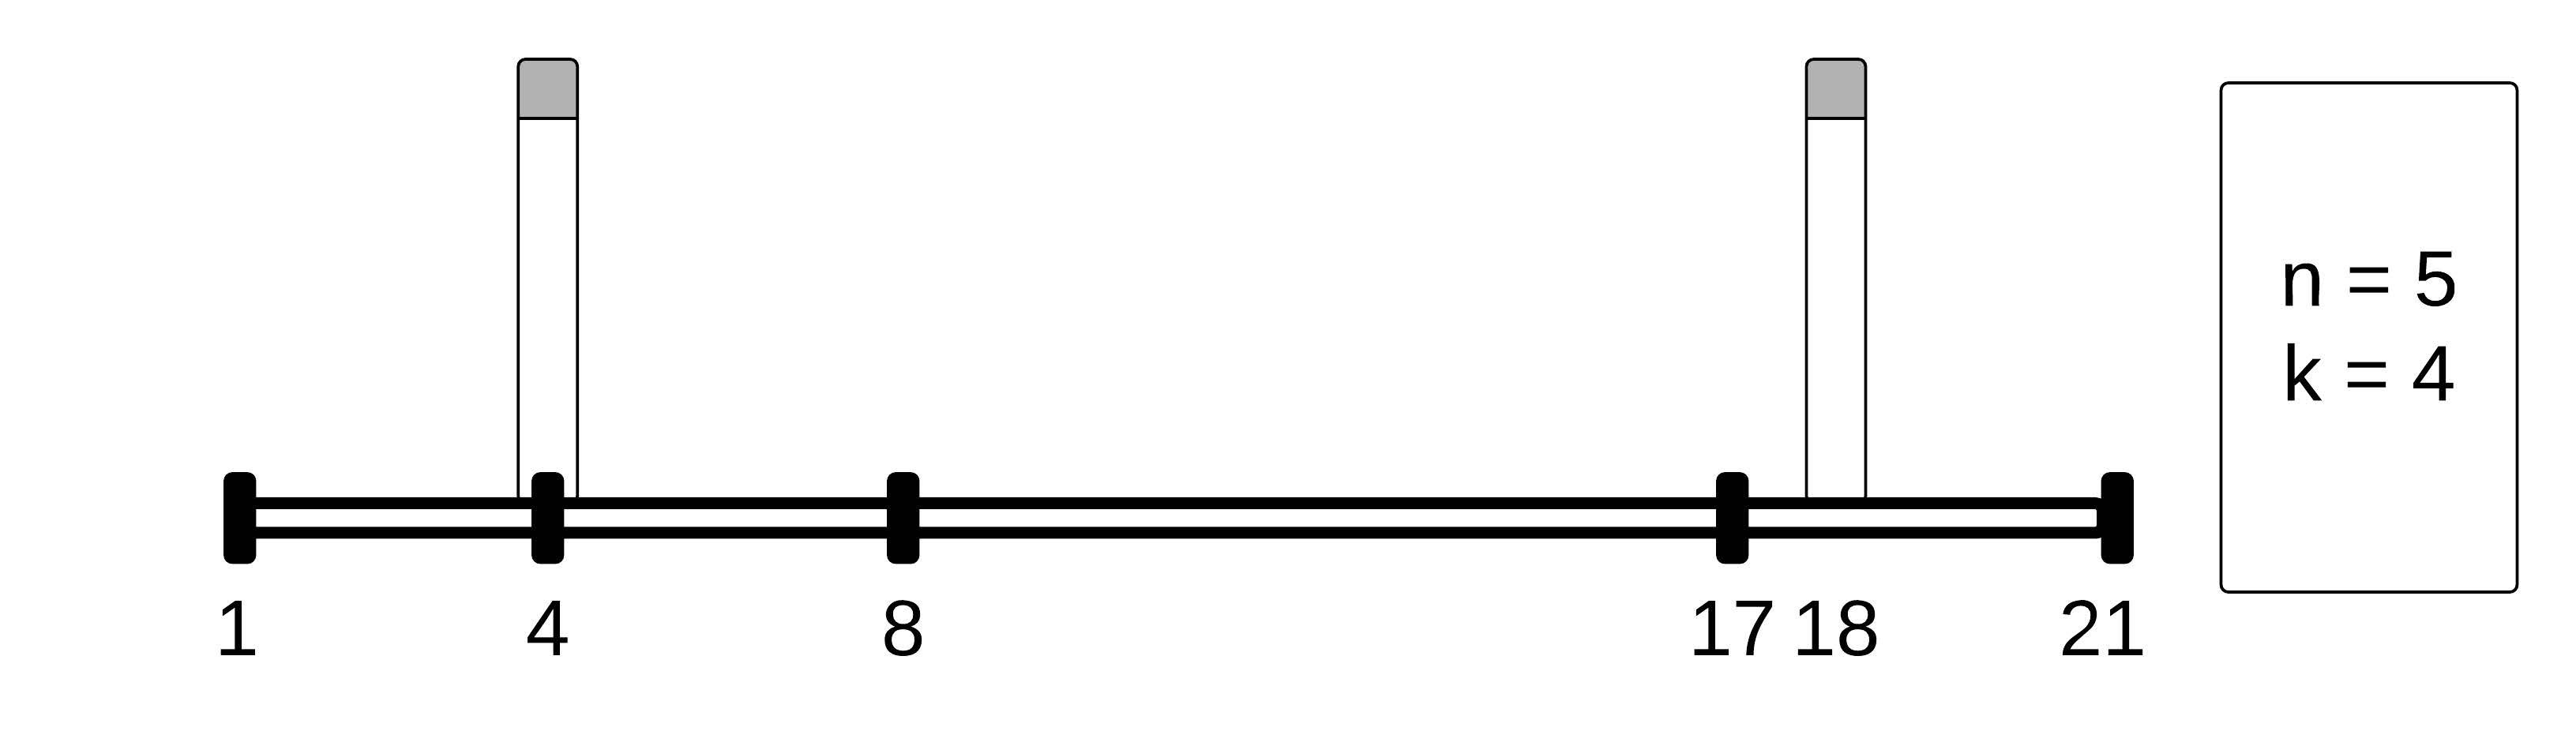
\includegraphics[width=0.7\textwidth]{Q5_2.jpg}
		\label{fig:Q5.2}
	\end{figure}

	\textit{Explanation}: In the above example, we have $n = 5, k = 4, x = [1, 4, 8, 17, 21]$. One of the optimal solution will use $2$ stalls, putting them at $x = 4$ and $x = 18$.
\end{enumerate}

\begin{solution}
\textbf{Please write down your solution to Problem 5 here.}
\end{solution}

\end{document}